You can activate Teststyle for a \gdproject{} in the \gdproject{} properties:

\begin{enumerate}
\item Open the \gdproject{} properties via: \\
\bxmenu{Test}{Properties}{}
\item Select \bxname{Teststyle} from the left.
\item Using the checkbox at the top of the dialog (\bxfigref{teststyle}), you can centrally activate or deactivate Teststyle for the whole \gdproject{}. 

\bxtipp{By default, Teststyle is activated for all \gdprojects{}.}

\item Click \bxcaption{OK} in the \gdproject{} properties to save the changes.
\item If your current \gdproject{} flouts any of the guidelines that are set, then you will see entries in the \gdprobview{} notifying you of the places where guidelines are being flouted. For more information on working with the \gdprobview{} to fix tests, see the section later \bxpref{TeststyleProbView}.

\bxtipp{The Teststyle settings are central for the whole \gdproject{} and will be seen by all users of the \gdproject{}.}

\end{enumerate}

\begin{figure}[p]
\begin{center}
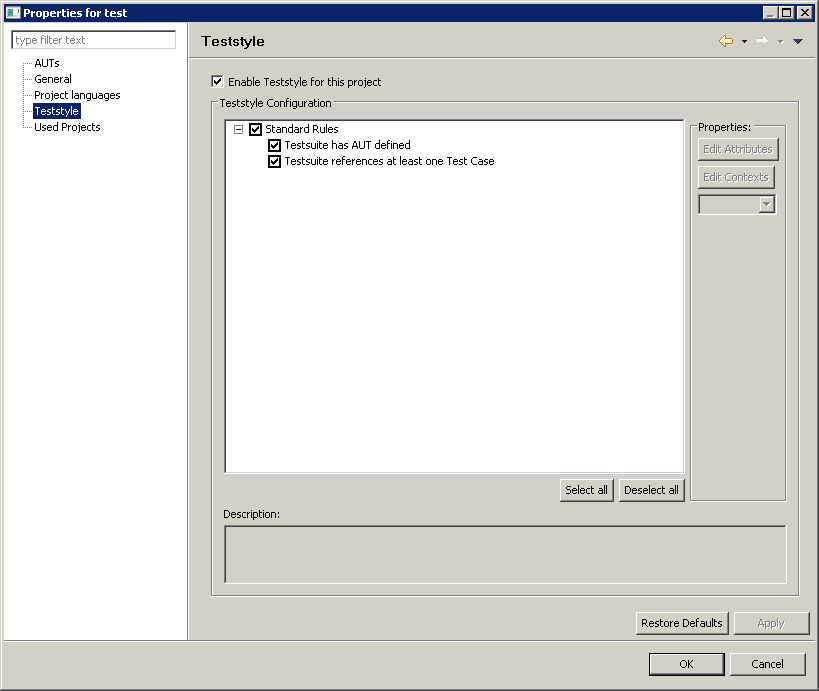
\includegraphics[width=12.5cm]{Tasks/Teststyle/PS/teststyle}
\caption{Teststyle}
\label{teststyle}
\end{center}
\end{figure}
